\documentclass[a4paper, 12pt]{article}

\usepackage{hyperref}
\usepackage[warn]{mathtext}
\usepackage[utf8]{inputenc}
\usepackage[T2A]{fontenc}
\usepackage[english,russian]{babel}
\usepackage{multirow}
\usepackage{float}
\restylefloat{table}
\usepackage{amsmath,amsfonts,amssymb,amsthm,mathtools}
\usepackage{indentfirst}
\DeclareSymbolFont{T2Aletters}{T2A}{cmr}{m}{it}
\usepackage{ gensymb }
\mathtoolsset{showonlyrefs=true}
\usepackage{euscript}
\usepackage{mathrsfs}
\usepackage[left=2cm,right=2cm,top=2cm,bottom=2cm]{geometry}
\usepackage{graphicx}
\usepackage{wrapfig}
\usepackage[rgb]{xcolor}
\hypersetup{
colorlinks=true,
urlcolor=blue
}
\usepackage{tikz}

\title{Лабораторная работа}
\author{Гисич Арсений Б03-102}
\date{2023}

\begin{document}

	\begin{center}
		{\large МОСКОВСКИЙ ФИЗИКО-ТЕХНИЧЕСКИЙ ИНСТИТУТ (НАЦИОНАЛЬНЫЙ ИССЛЕДОВАТЕЛЬСКИЙ УНИВЕРСИТЕТ)}
	\end{center}
	\vspace{5 cm}
	{\Large
		\begin{center}
			{\bf Лабораторная работа 4.7.2}\\[0.2 cm]
			Эффект Поккельса
		\end{center}
	}
	\vspace{4 cm}
	\begin{flushright}
		{\Large Выполнили: \\
			\vspace{0.2 cm}
			Гисич Арсений \\
                Айрапетян Микаел \\ 
			\vspace{0.2 cm}
			Б03-102 \\}
	\end{flushright}
	\vspace{8 cm}
	\begin{center}
		Долгопрудный\\[0.1 cm]
		2023
	\end{center}
\thispagestyle{empty}

\section{Аннотация}

В данной работе по измерениям радиусов интерференционных колец была определена разность показателей преломления $n_o - n_e$; путём подачи на кристалл постоянного напряжения был получен свет, поляризованный по кругу; было определено полуволновое напряжение по фигурам Лиссажу на экране осциллографа.

\section{Теоретические сведения}

Эффект Поккельса --- изменение показателя преломления света в кристалле под действием электрического поля.\\
Рассмотрим кристалл ниобата лития $\text{LiNbO}_3$ с центрально-осевой симметрией вдоль оси $Z$. Для световой волны с $\mathbf{E}$ перпендикулярно $Z$ показатель преломления будет $n_o$, а для волны с $\mathbf{E}$ вдоль $Z$ --- $n_e$. В случае, когда луч света идёт под углом $\theta$ к оси, есть два значение показателя преломления $n_1$ и $n_2$: $n_1 = n_o$ для волны с $\mathbf{E}$ перпендикулярным плоскости $(\mathbf{k},\mathbf{Z})$ (обыкновенная волна) и $n_2$ для волны с $\mathbf{E}$ в этой плоскости (необыкновенная волна). В последнем случае
\begin{equation}
\dfrac{1}{n_2^2}=\dfrac{\cos^2 \theta}{n_0^2}+\dfrac{\sin^2 \theta}{n_e^2}.
\end{equation}

\begin{figure}[H]
\begin{center}
    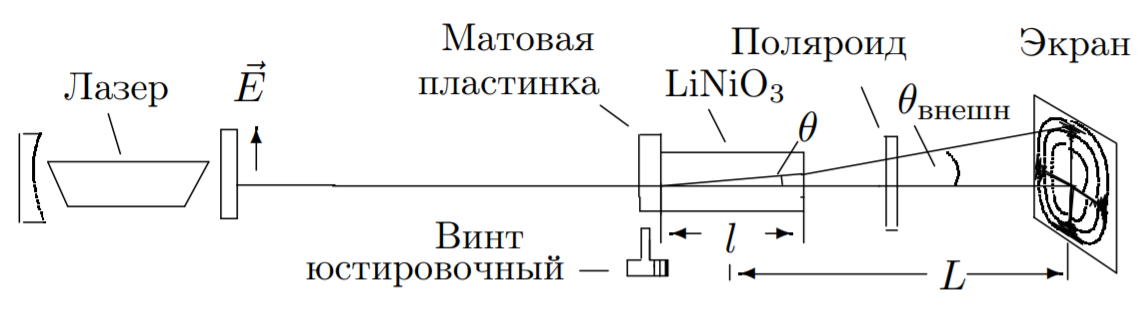
\includegraphics[width=1\linewidth]{1.png}
\end{center}
\caption{Схема для наблюдения интерференционной картины}
\label{fig:scheme_interfer}
\end{figure}

Если перед кристаллом, помещённым между поляроидами, расположить линзу или матовую пластинку, то на экране за поляроидом мы увидим тёмные концентрические окружности --- результат интерференции обыкновенной и необыкновенной волн. При повороте выходного поляроида на $90^\circ$ картина меняется с позитива на негатив (на месте светлых пятен тёмные и наоборот). В случаи, когда разрешённое направление анализатора перпендикулярно поляризации лазерного излучения, радиус тёмного кольца с номером $m$ равен
\begin{equation}\label{eq:2-luch}
r_m^2 = \dfrac{\lambda}{l} \dfrac{(n_oL)^2}{n_0 - n_e}m,
\end{equation}
где $L$ --- расстояние от центра кристалла до экрана, $l$ --- длина кристалла.\\
Теперь поместим кристалл в постоянное электрическое поле $E_{\text{эл}}$, направленное вдоль оси $X$, перпендикулярной $Z$. Показатель преломления для луча, распространяющего вдоль $Z$, всегда $n_o$. В плоскости $(X,Y)$ возникают два главных направления под углами $45^\circ$ к $X$ и $Y$ с показателями преломления $n_0 - \Delta n$ и $n_o + \Delta n$ (быстрая и медленная ось), причём $\Delta n = A E_{\text{эл}}$. Для поляризованного вертикально света и анализатора, пропускающего горизонтальную поляризацию, на выходе интенсивность на выходе будет иметь вид
\begin{equation}
I_{\text{вых}} = I_0 \sin^2 \left(\dfrac{\pi}{2} \dfrac{U}{U_{\lambda/2}} \right),
\end{equation}
где $U_{\lambda/2} = \frac{\lambda}{4A}\frac{d}{l}$ --- \textit{полуволновое напряжение}, $d$ --- поперечный размер кристалла.  При напряжении $U = E_{\text{эл}}d$ равном полуволновому сдвиг фаз между двумя волнами равен $\pi$, а интенсивность света на выходе максимальна. 


\begin{figure}[H]
\begin{center}
    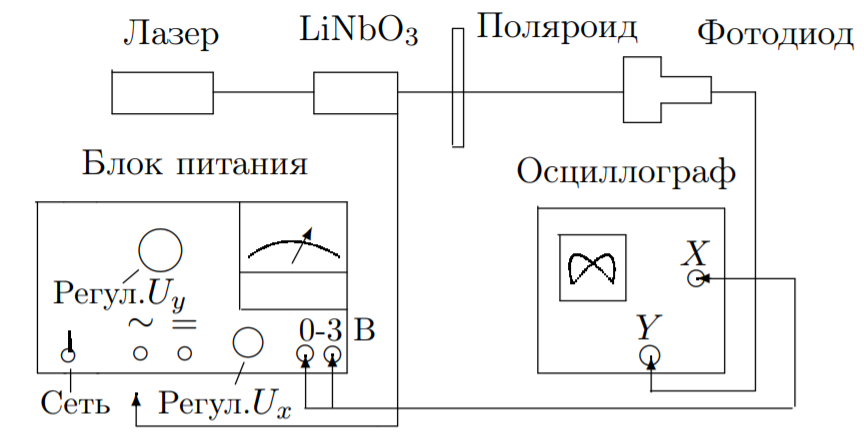
\includegraphics[scale=0.7]{2.png}
\end{center}
\caption{Схема установки.}
\label{fig:scheme}
\end{figure}

На Рис. 2 представлена схема всей установки (оптическая часть изображена на Рис. 1). Свет лазера, проходя через сквозь пластину, рассеивается и падает на двояко-преломляющий кристалл. На экране за поляроидом видна интерференционная картина. Убрав рассеивающую пластину и подавая на кристалл постоянное напряжение, можно величиной напряжения влиять на поляризацию луча, вышедшего из кристалла. Заменив экран фотодиодом и подав на кристалл переменное напряжение, можно исследовать поляризацию с помощью осциллографа.
	
\newpage

\section{Используемое оборудование}

\begin{enumerate}
    \item гелий-неоновый лазер;
    \item поляризатор;
    \item кристалл ниобата лития;
    \item матовая пластина;
    \item экран;
    \item источник высоковольтного переменного и постоянного напряжения;
    \item фотодиод;
    \item осциллограф;
    \item линейка.
\end{enumerate}

\section{Результаты измерений и обработка данных}

Параметры установки:
\begin{description}
\item{} $n_o = 2,29$
\item{} $l = 26~мм$
\item{} $\lambda = 0,63~мкм$
\item{} $L = 75\pm0,5~см$
\end{description}

Результаты измерений радиуса тёмных колец $r(m)$ представлены в таб.~\ref{tab1}. График зависимости $r^2 = f(m)$ представлен на рис.~\ref{plot1}.

\begin{table}[h!]
\begin{center}
\begin{tabular}{|c|c|c|}
\hline
$m$ & $r(m), см$ & $\delta_{r(m)}, см$ \\ \hline
1 & 2,7      & 0,1       \\ \hline
2 & 4,0      & 0,1       \\ \hline
3 & 4,7      & 0,1       \\ \hline
4 & 5,5      & 0,1       \\ \hline
5 & 6,2      & 0,1       \\ \hline
6 & 6,7      & 0,1       \\ \hline
\end{tabular}
\end{center}
\caption{Зависимость радиуса тёмных колец от номера кольца}
\label{tab1}
\end{table}

\begin{figure}[h!]
\begin{center}
    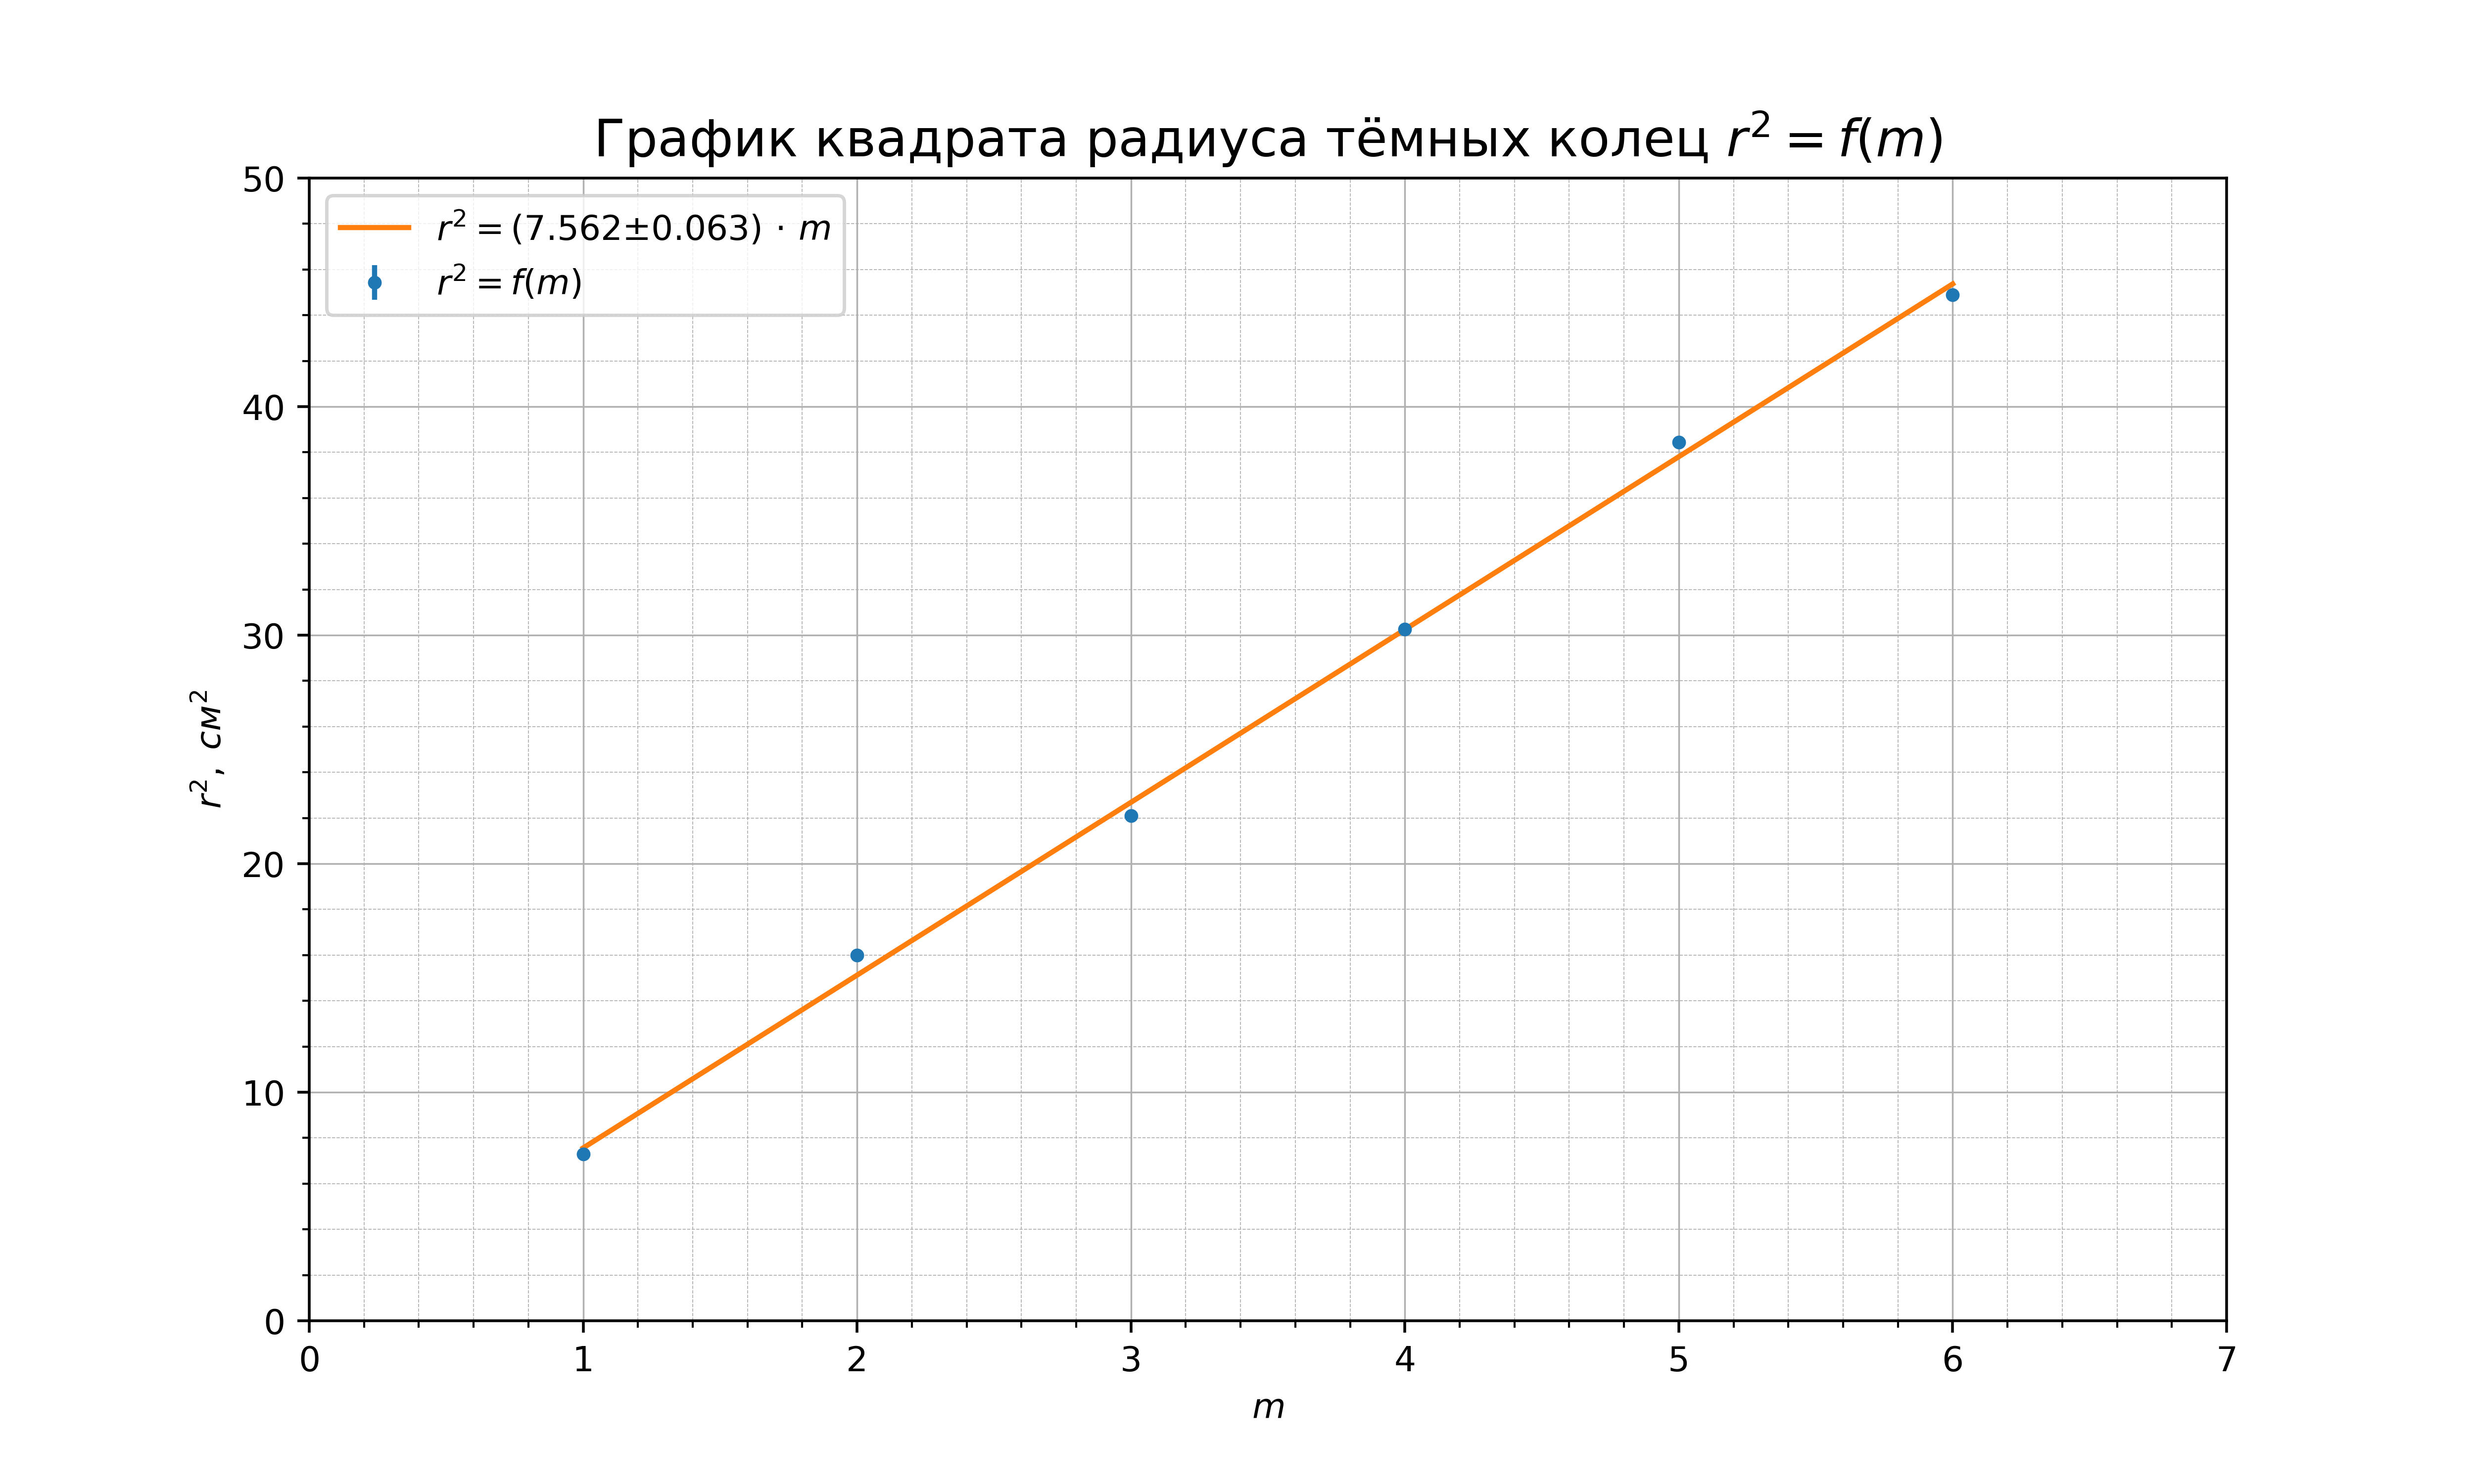
\includegraphics[scale=0.7]{4.7.2_1.png}
\end{center}
\caption{График функции зависимости квадрата радиуса кольца от его номера $r^2 = f(m)$}
\label{plot1}
\end{figure}

Угол наклона графика $k = 7,562\pm0,063~см^2$. Из формулы \eqref{eq:2-luch} определяем двулучепреломление ниобата лития $(n_o - n_e) = \frac{\lambda}{l}\frac{(n_o L)^2}{k} = (94,5\pm1,5)~\cdot~10^{-3}$.

\newpage

При постоянном напряжении на кристалле определяется полуволновое напряжение. Полученное значение при скрещенной поляризации: $U_{\lambda/2} = 0,42\pm0,01~кВ$, а при параллельной: $U_{\lambda/2} = 0,39\pm0,01~кВ$.

Заменим в схеме, изображенной на рисунке \ref{fig:scheme}, экран фотодиодом, подключим его к $Y$-входу осциллографа. На $X$-вход подадим переменное напряжение с блока питания. В режиме DUAL на экране осциллографа получаются фигуры Лиссажу, отвечающие зависимости $I(U)$. Для скрещенных поляризаций имеет вид синусоиды, взятой на симметричном отрезке, а для параллельных поляризаций представляет собой косинусоиду. Таким образом, фигуры Лиссажу для разных поляризаций при одинаковом значении амплитуды напряжения $U$ отличаются по фазе на $\pi/2$.
	
Определим полуволновое напряжение, измерив разность показаний между последовательными фигурами Лиссажу на экране, соответствующие экстремумам сигнала: 
	
\[ U_{\lambda/2} \approx 30 \text{ дел} = 450 \text{ В} \]
	
Фотографии наблюдаемых фигур Лиссажу для напряжений, кратным полуволновому, при разных поляризациях представлены на рисунке \ref{lis}.
	
	
	\begin{figure}[h]
		\begin{minipage}[h]{0.3\linewidth}
			\center{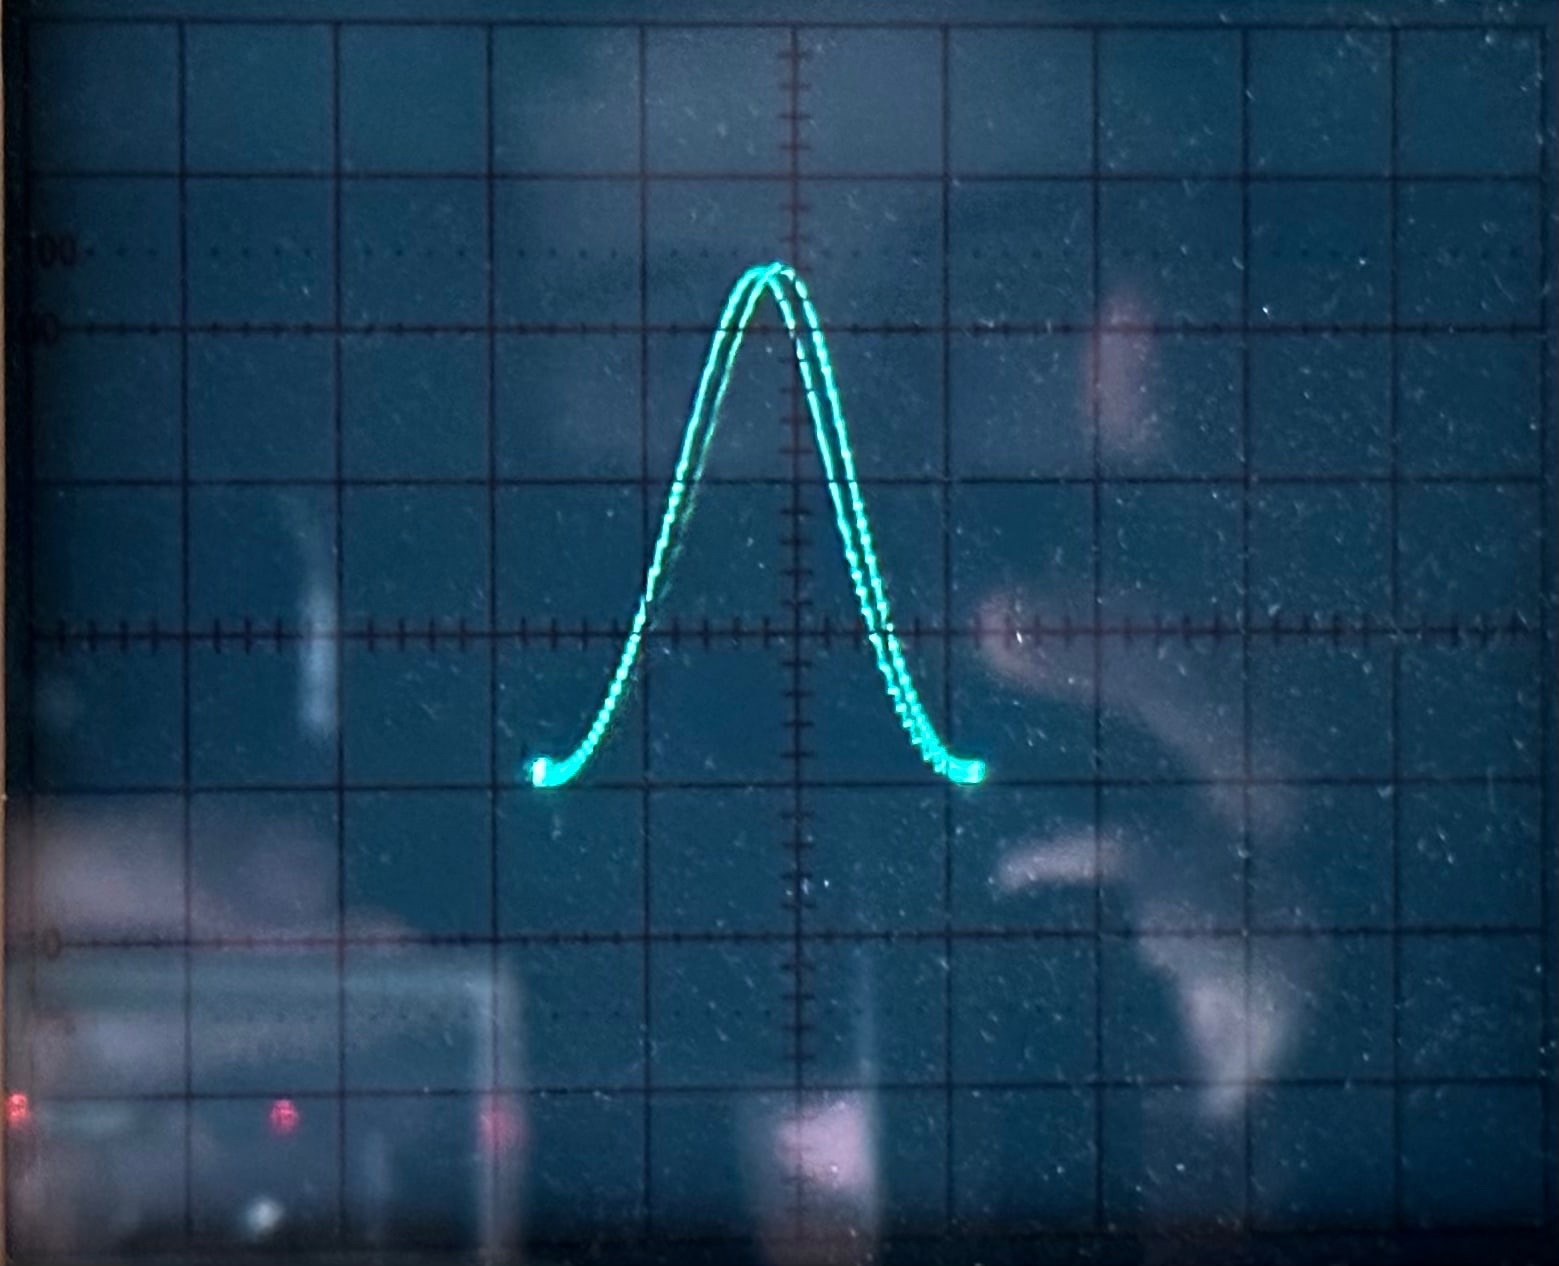
\includegraphics[width=0.9\linewidth]{sin1.jpg} \\ a)}
		\end{minipage}
		\hfill
		\begin{minipage}[h]{0.3\linewidth}
			\center{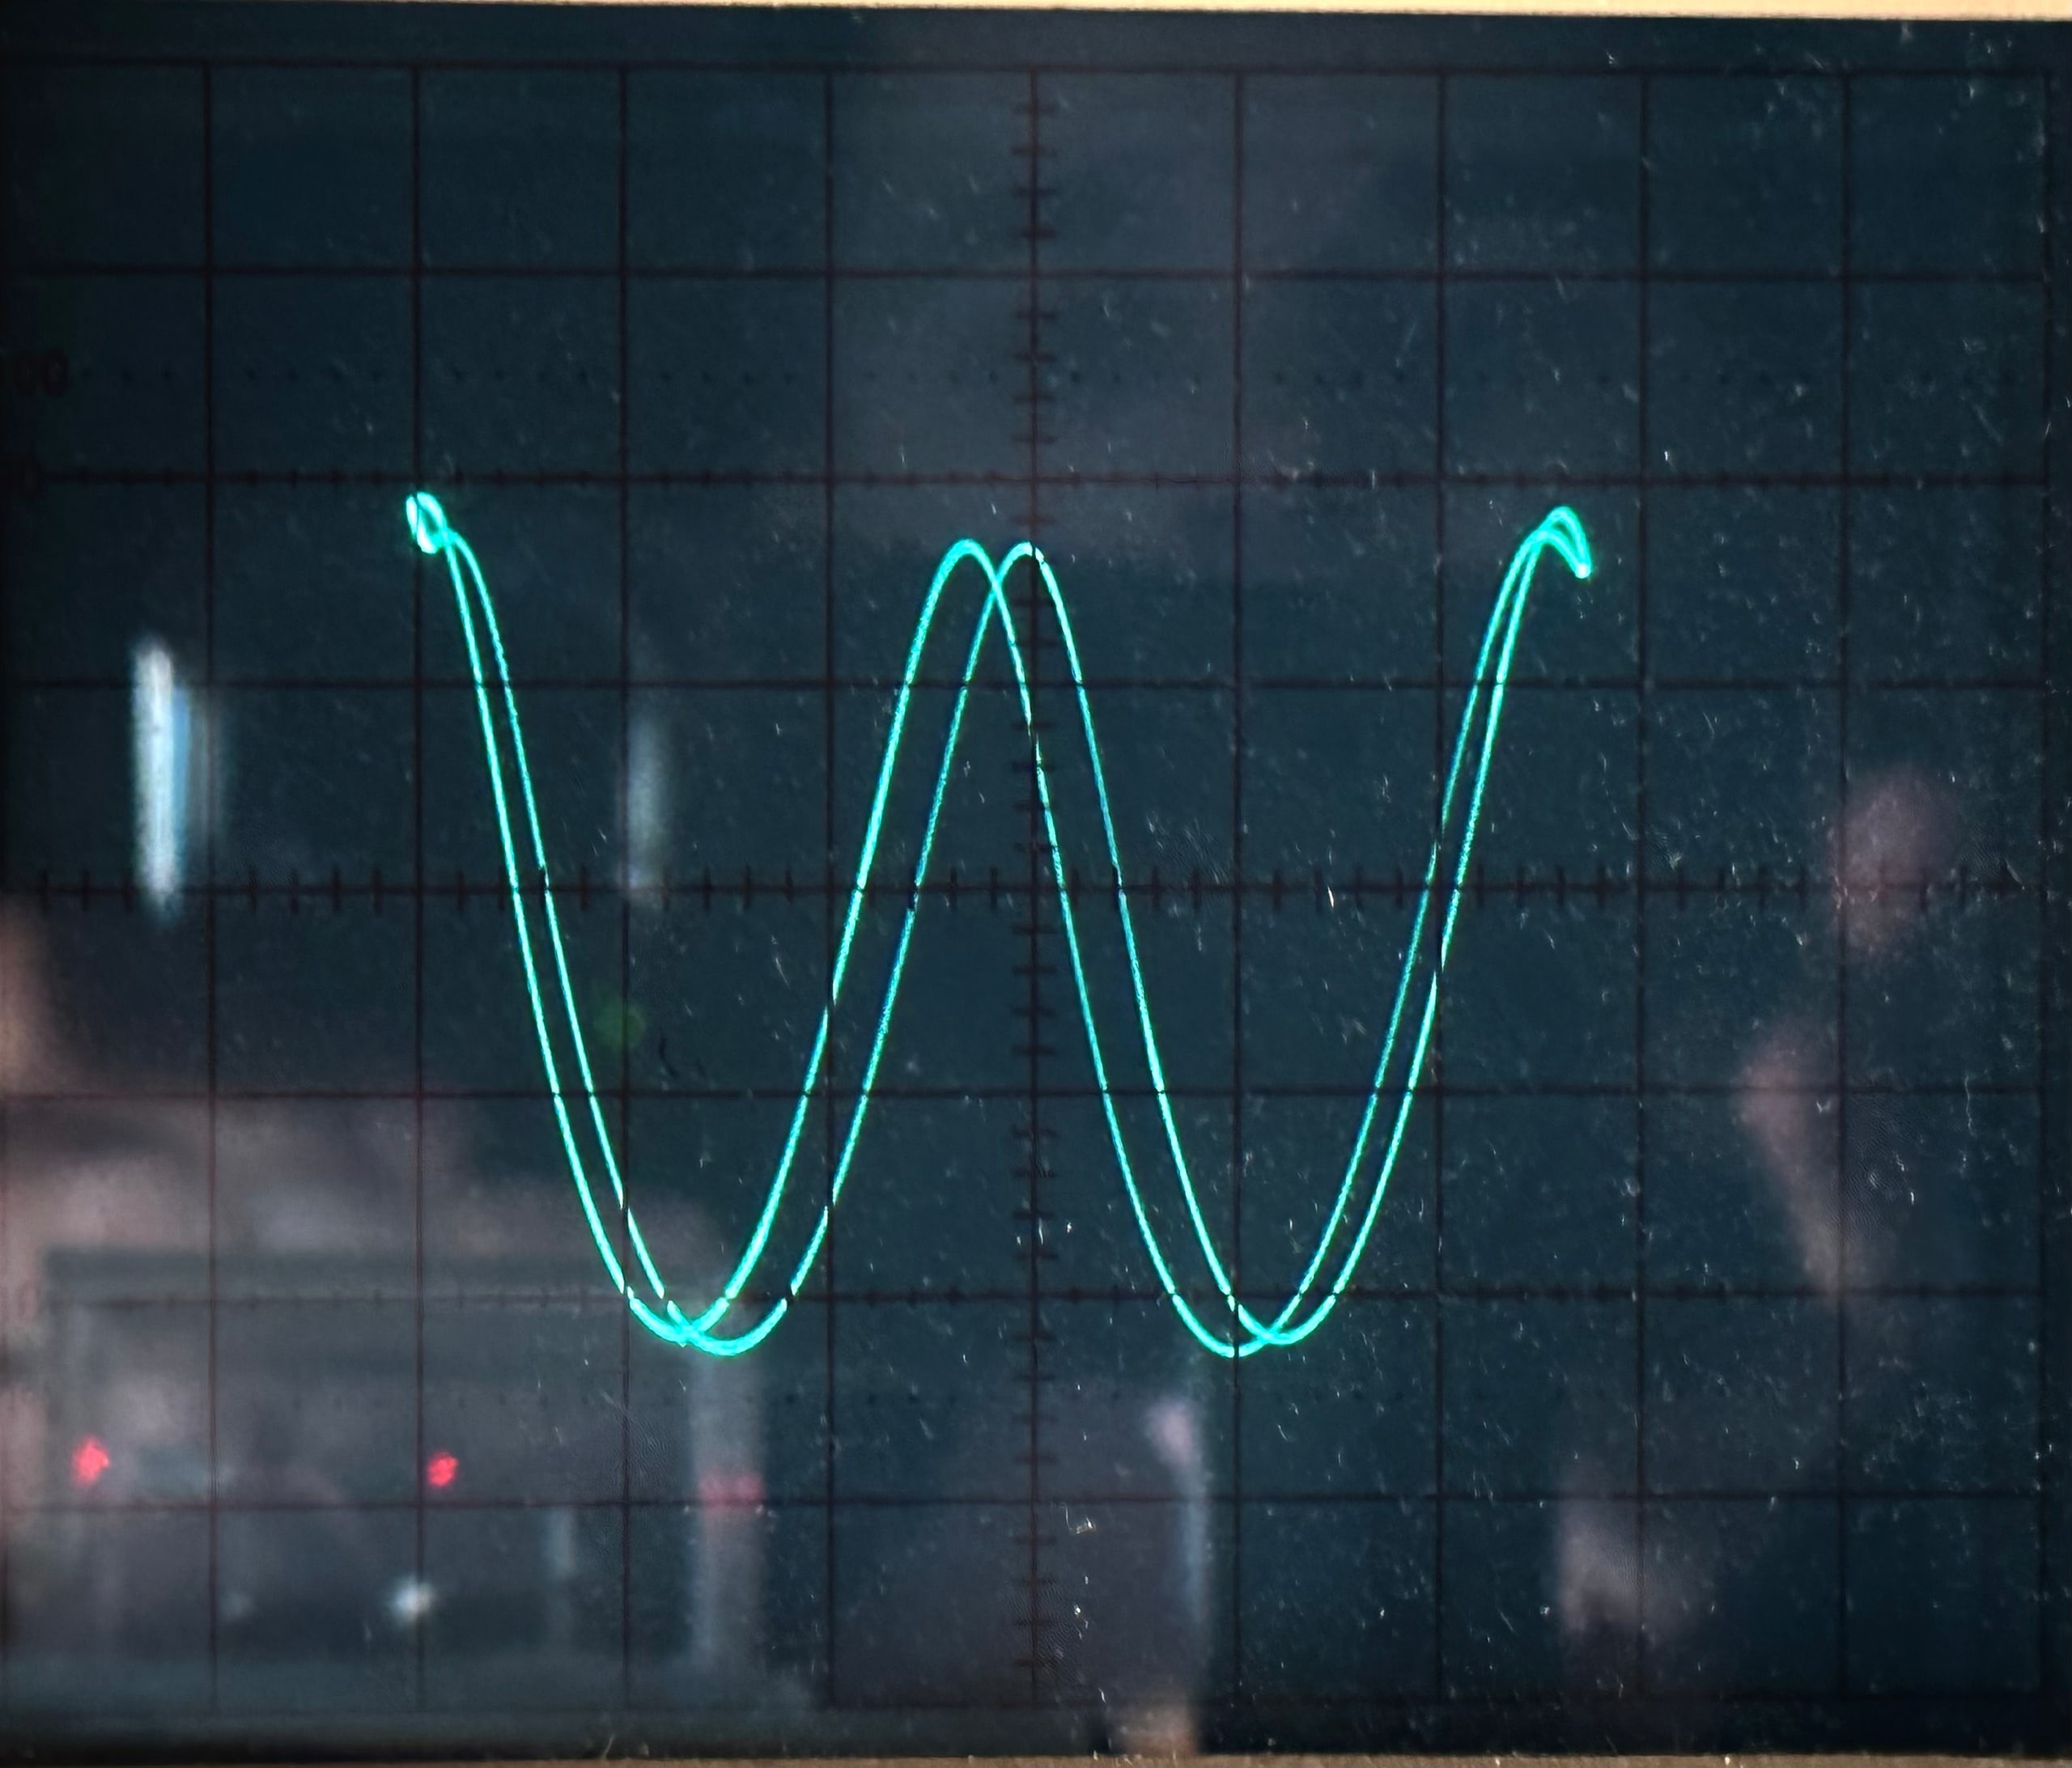
\includegraphics[width=0.9\linewidth]{sin2.jpg} \\ b)}
		\end{minipage}
		\hfill
		\begin{minipage}[h]{0.3\linewidth}
			\center{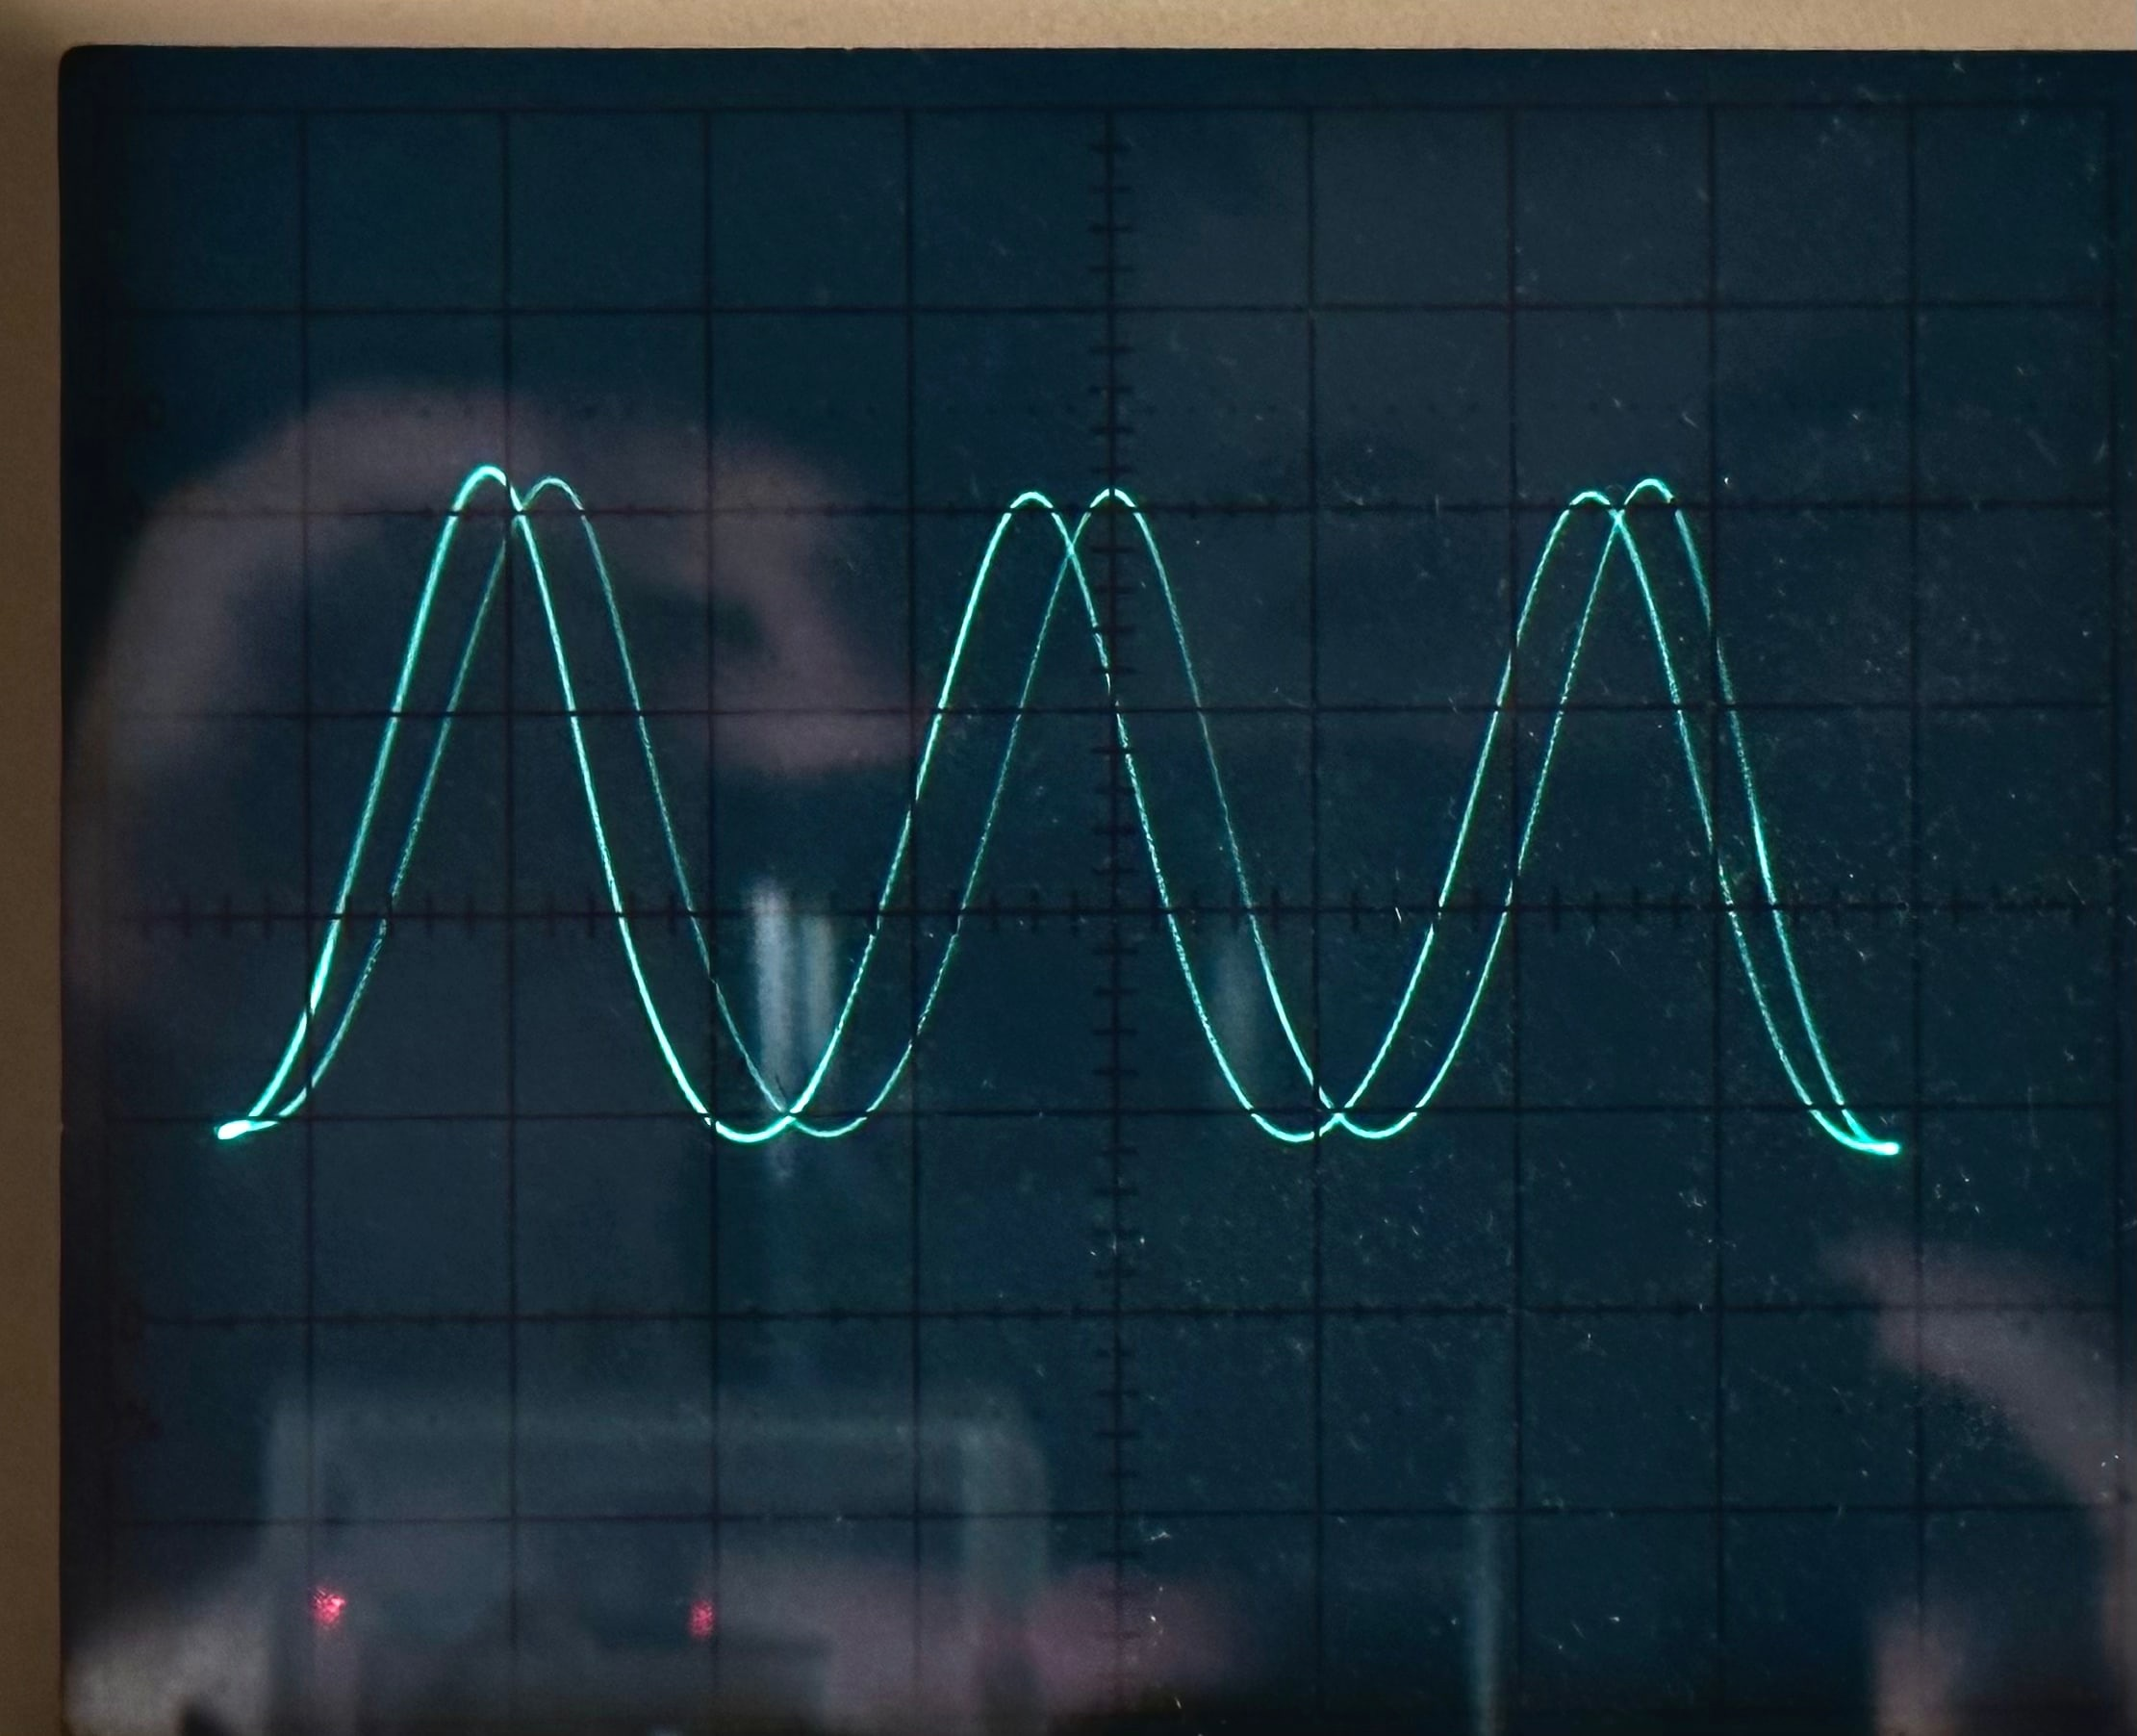
\includegraphics[width=0.9\linewidth]{sin3.jpg} \\ c)}
		\end{minipage}
		\caption{Фигуры Лиссажу для скрещенных поляризаций при различных амплитудах напряжения $U$: (a) $U = U_{\lambda/2}$, (b) $U = U_{\lambda}$, (c) $U = U_{3\lambda/2}$ }
		\label{lis}
	\end{figure}
 
 %%%%%%%%%%%%%%%%%%%%%%%%%%%%%%%%%%%%%%%%%
 
	\begin{figure}[h]
		\begin{minipage}[h]{0.3\linewidth}
			\center{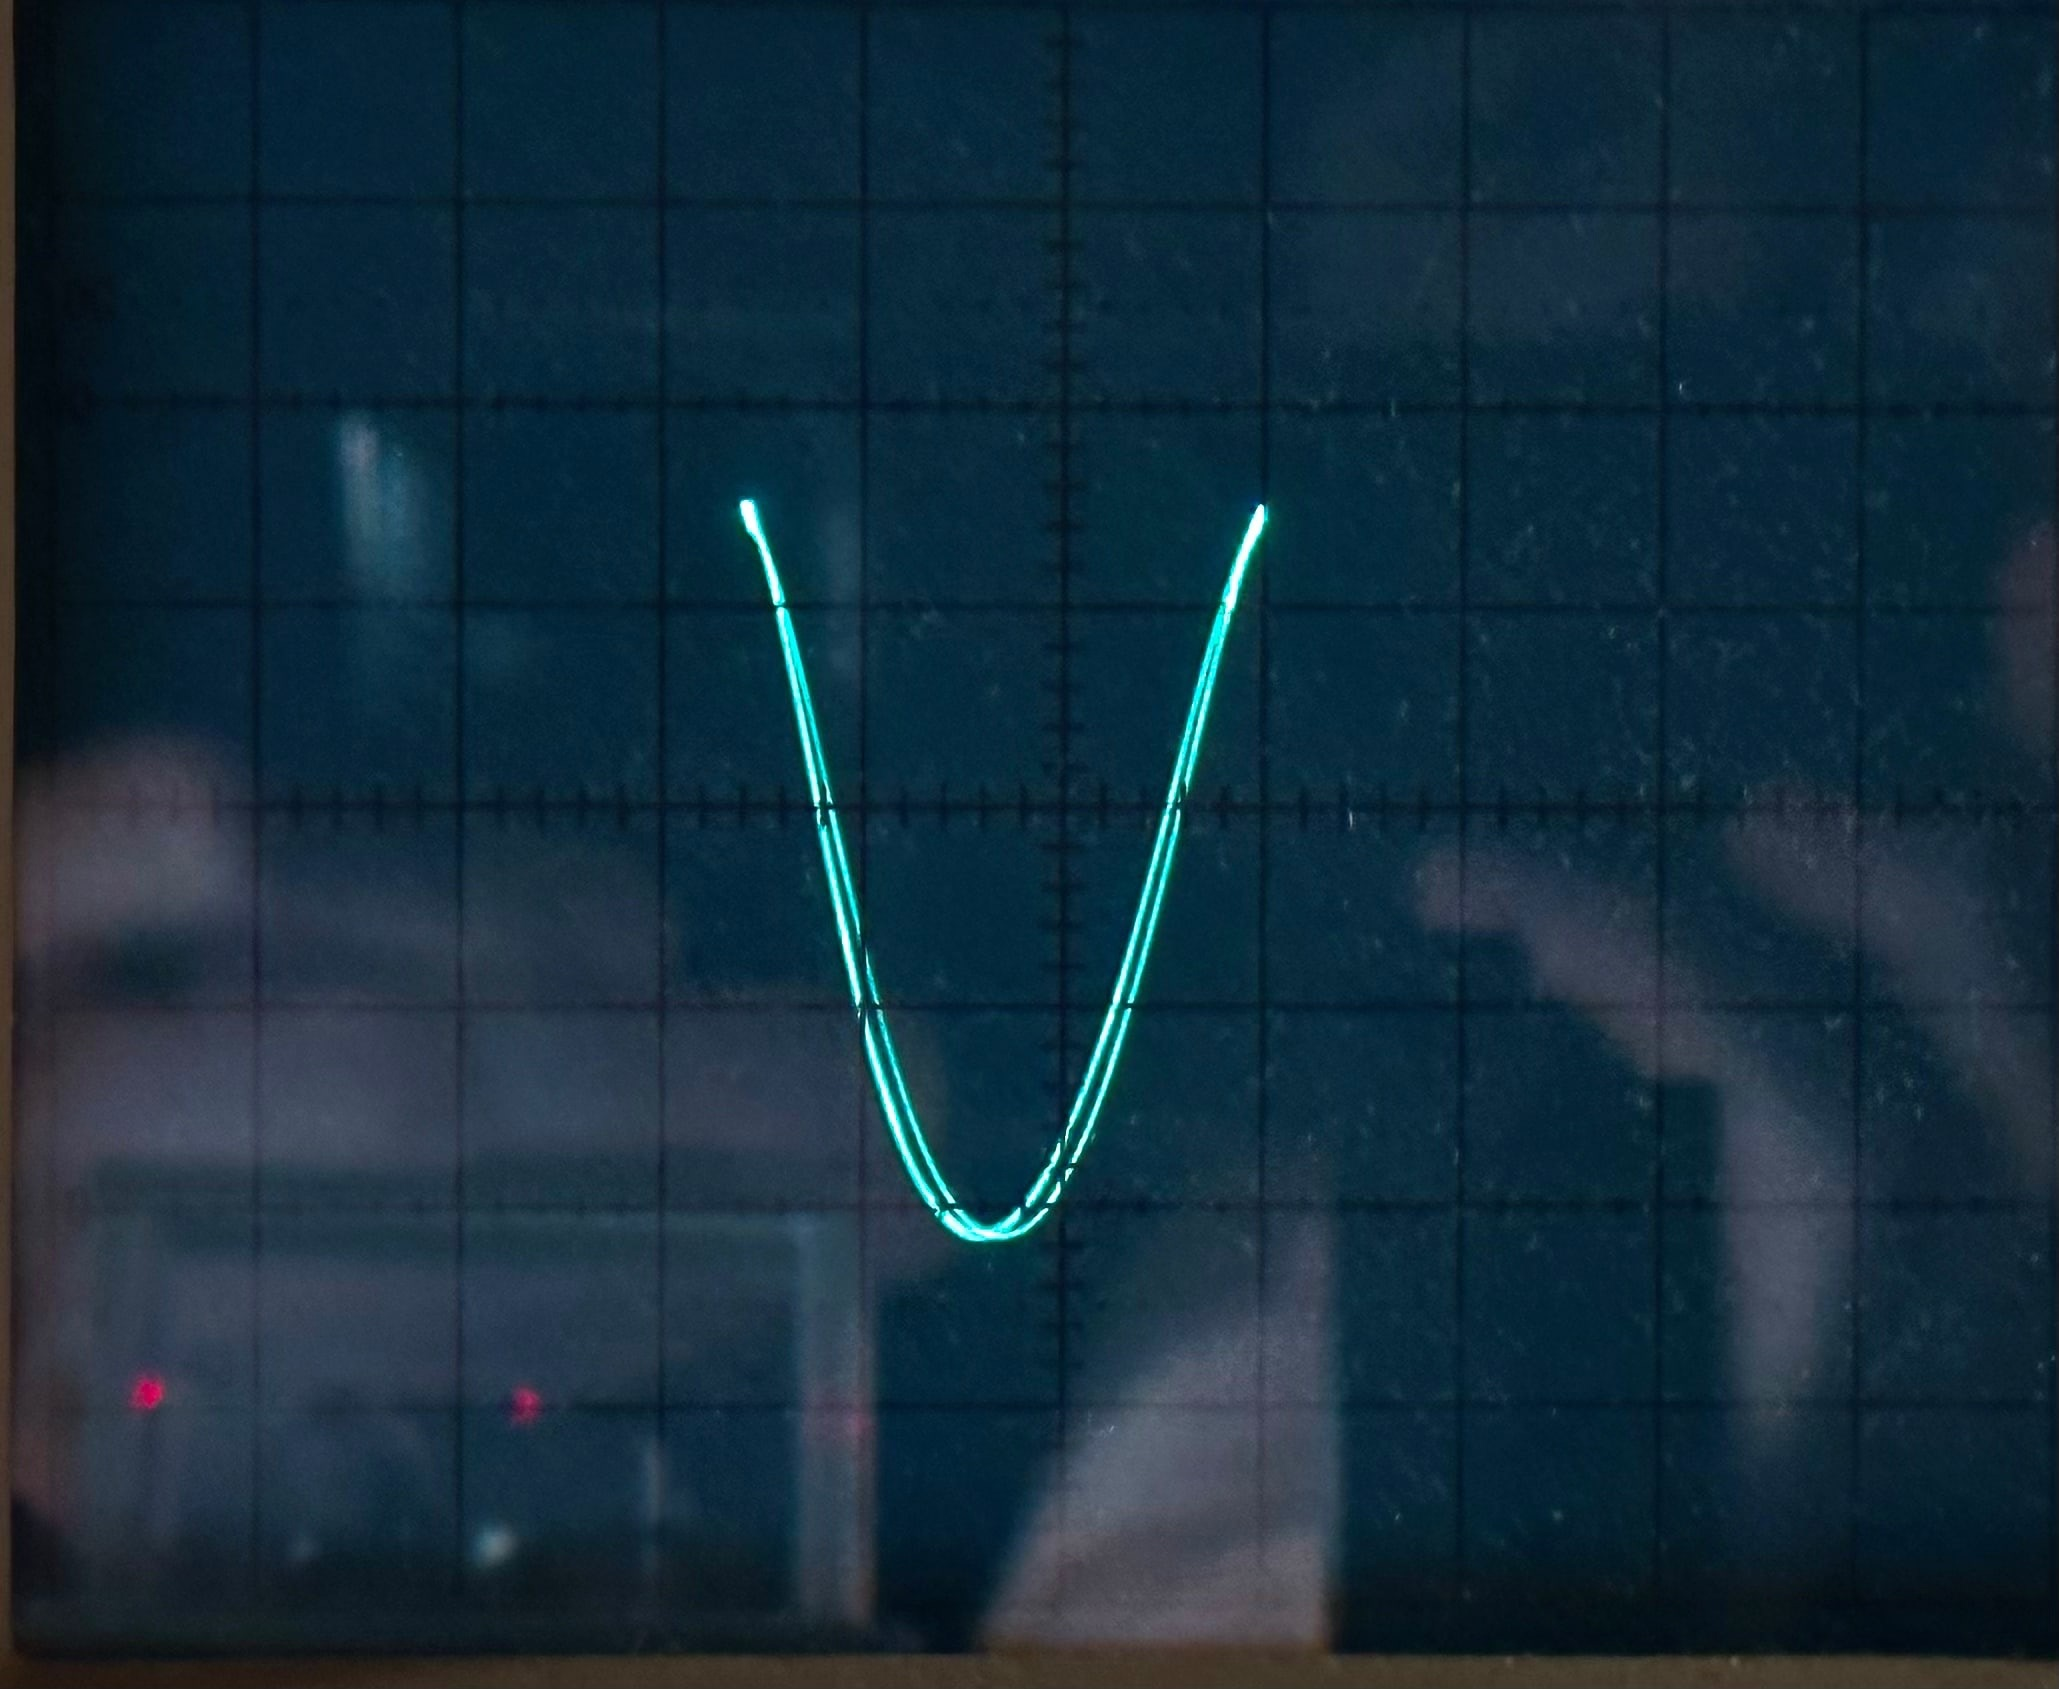
\includegraphics[width=0.9\linewidth]{cos1.jpg} \\ a)}
		\end{minipage}
		\hfill
		\begin{minipage}[h]{0.3\linewidth}
			\center{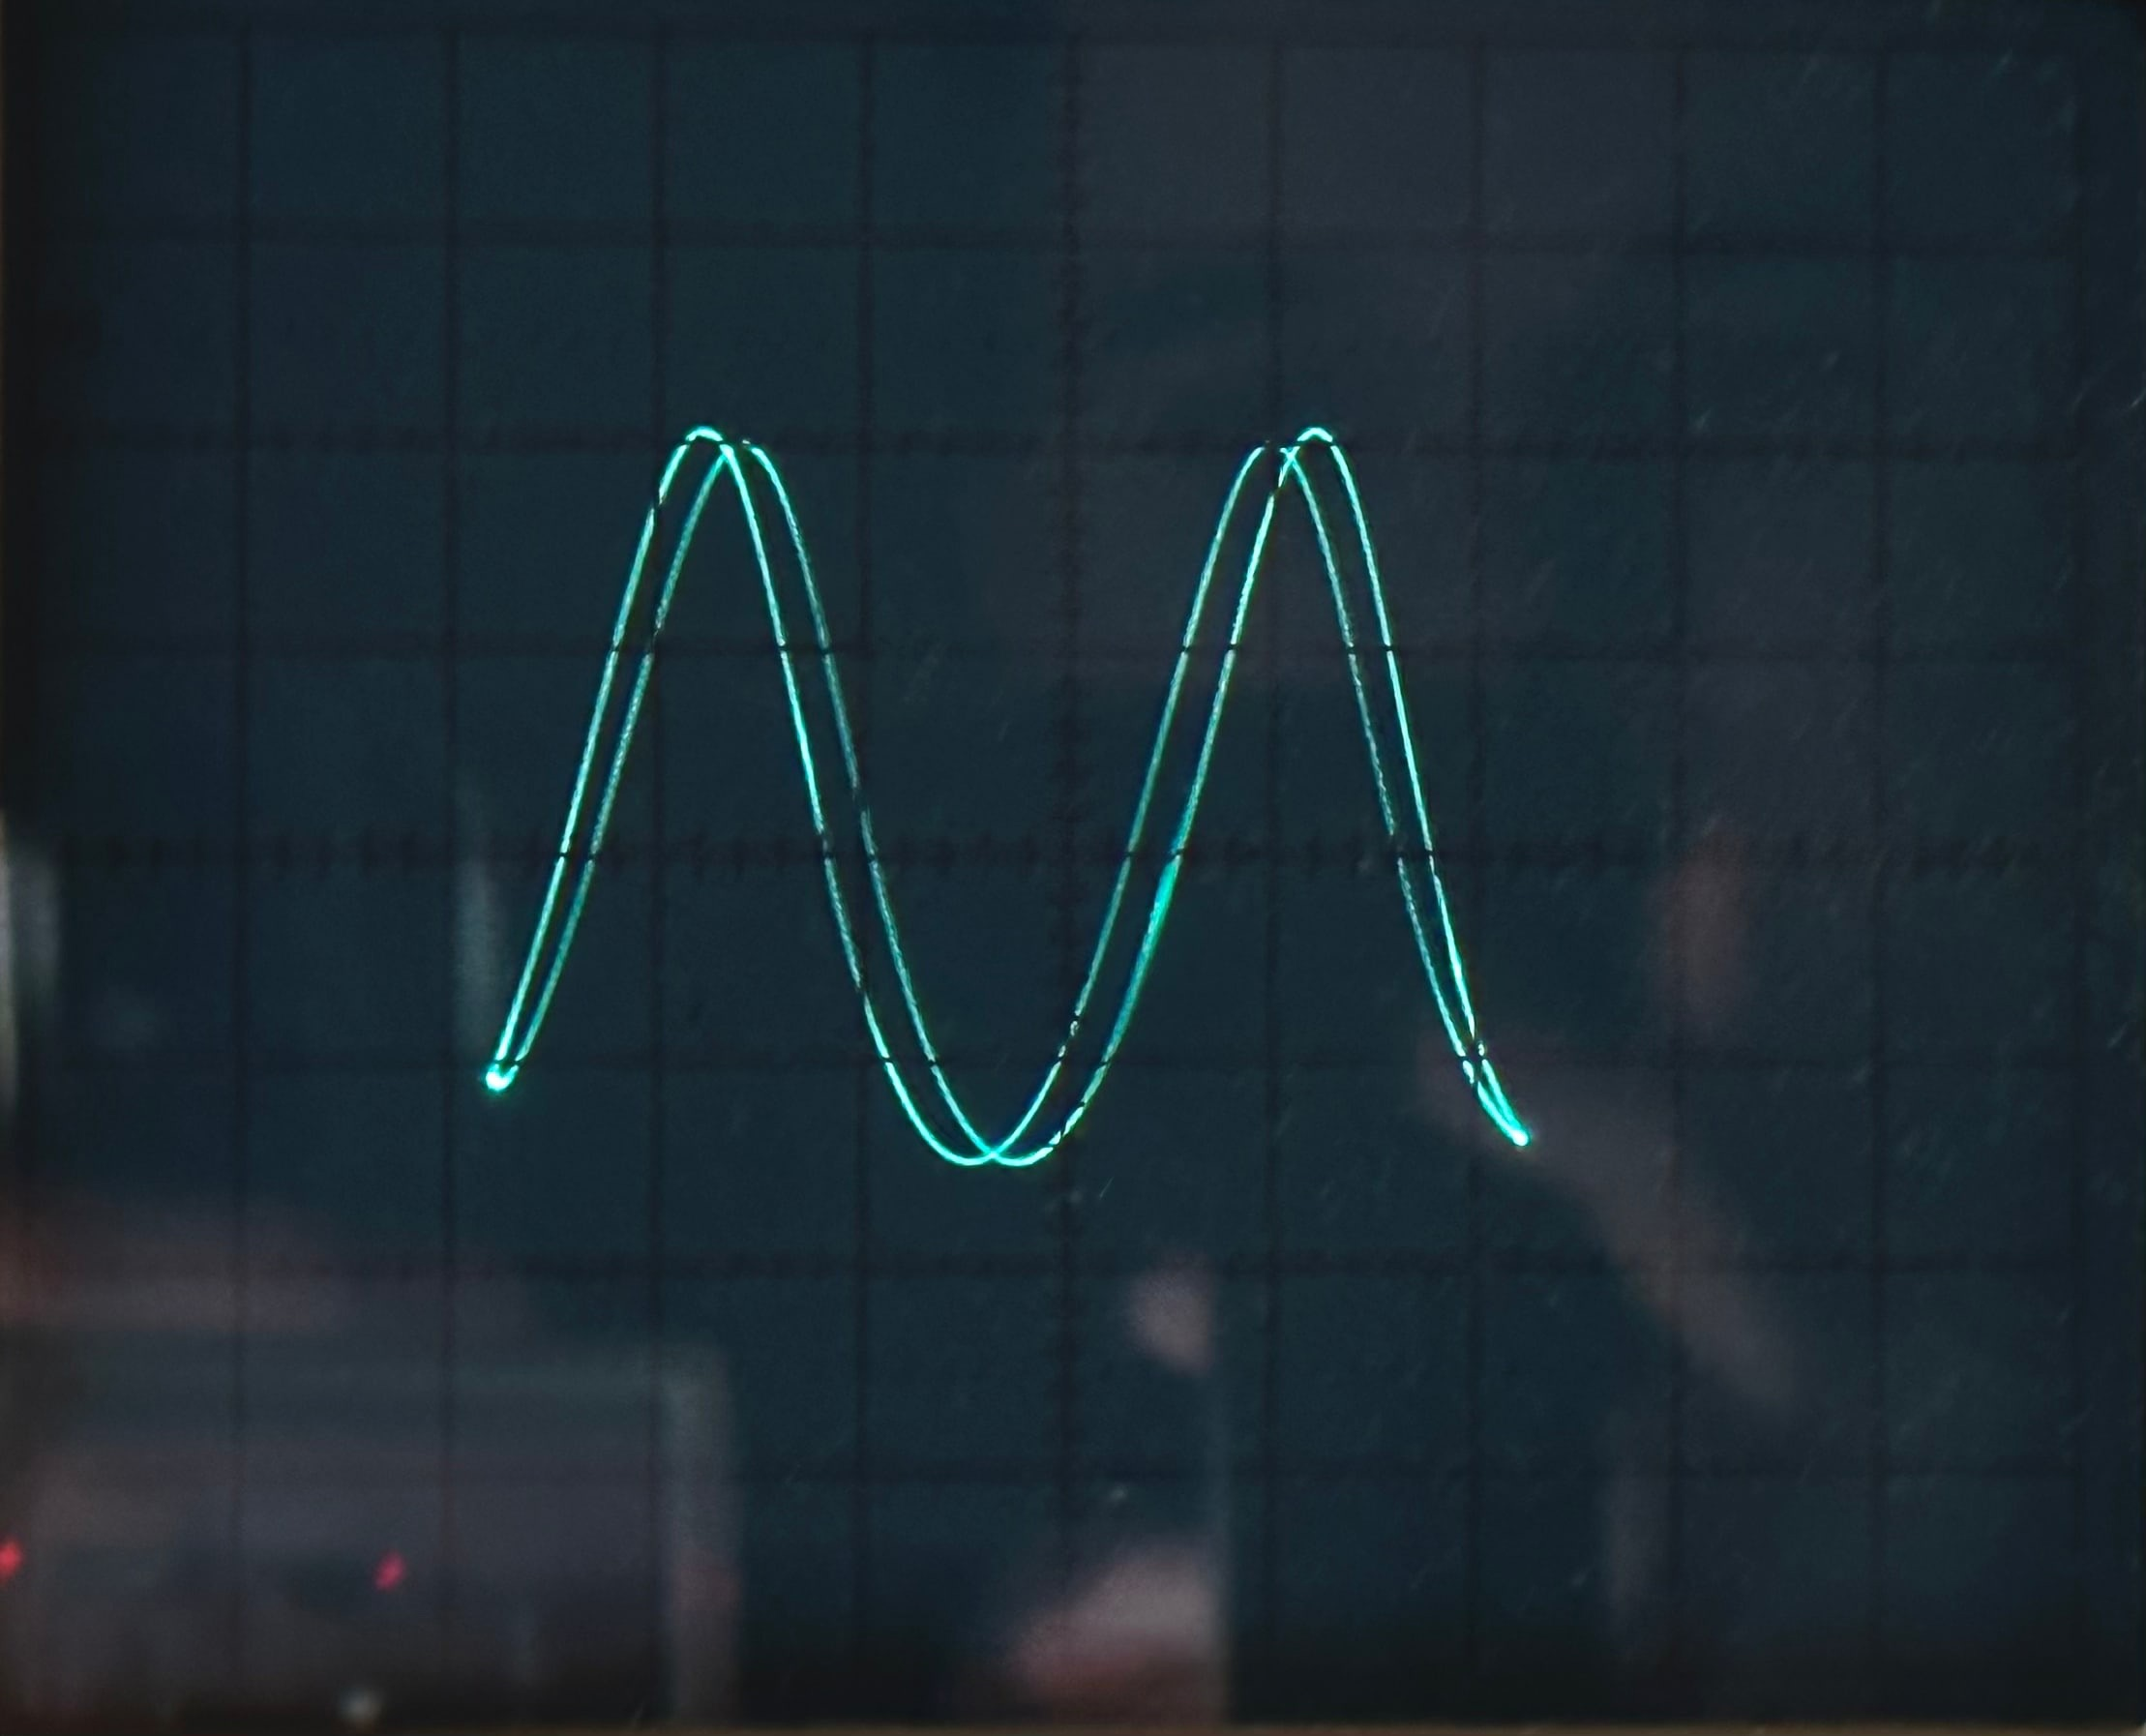
\includegraphics[width=0.9\linewidth]{cos2.jpg} \\ b)}
		\end{minipage}
		\hfill
		\begin{minipage}[h]{0.3\linewidth}
			\center{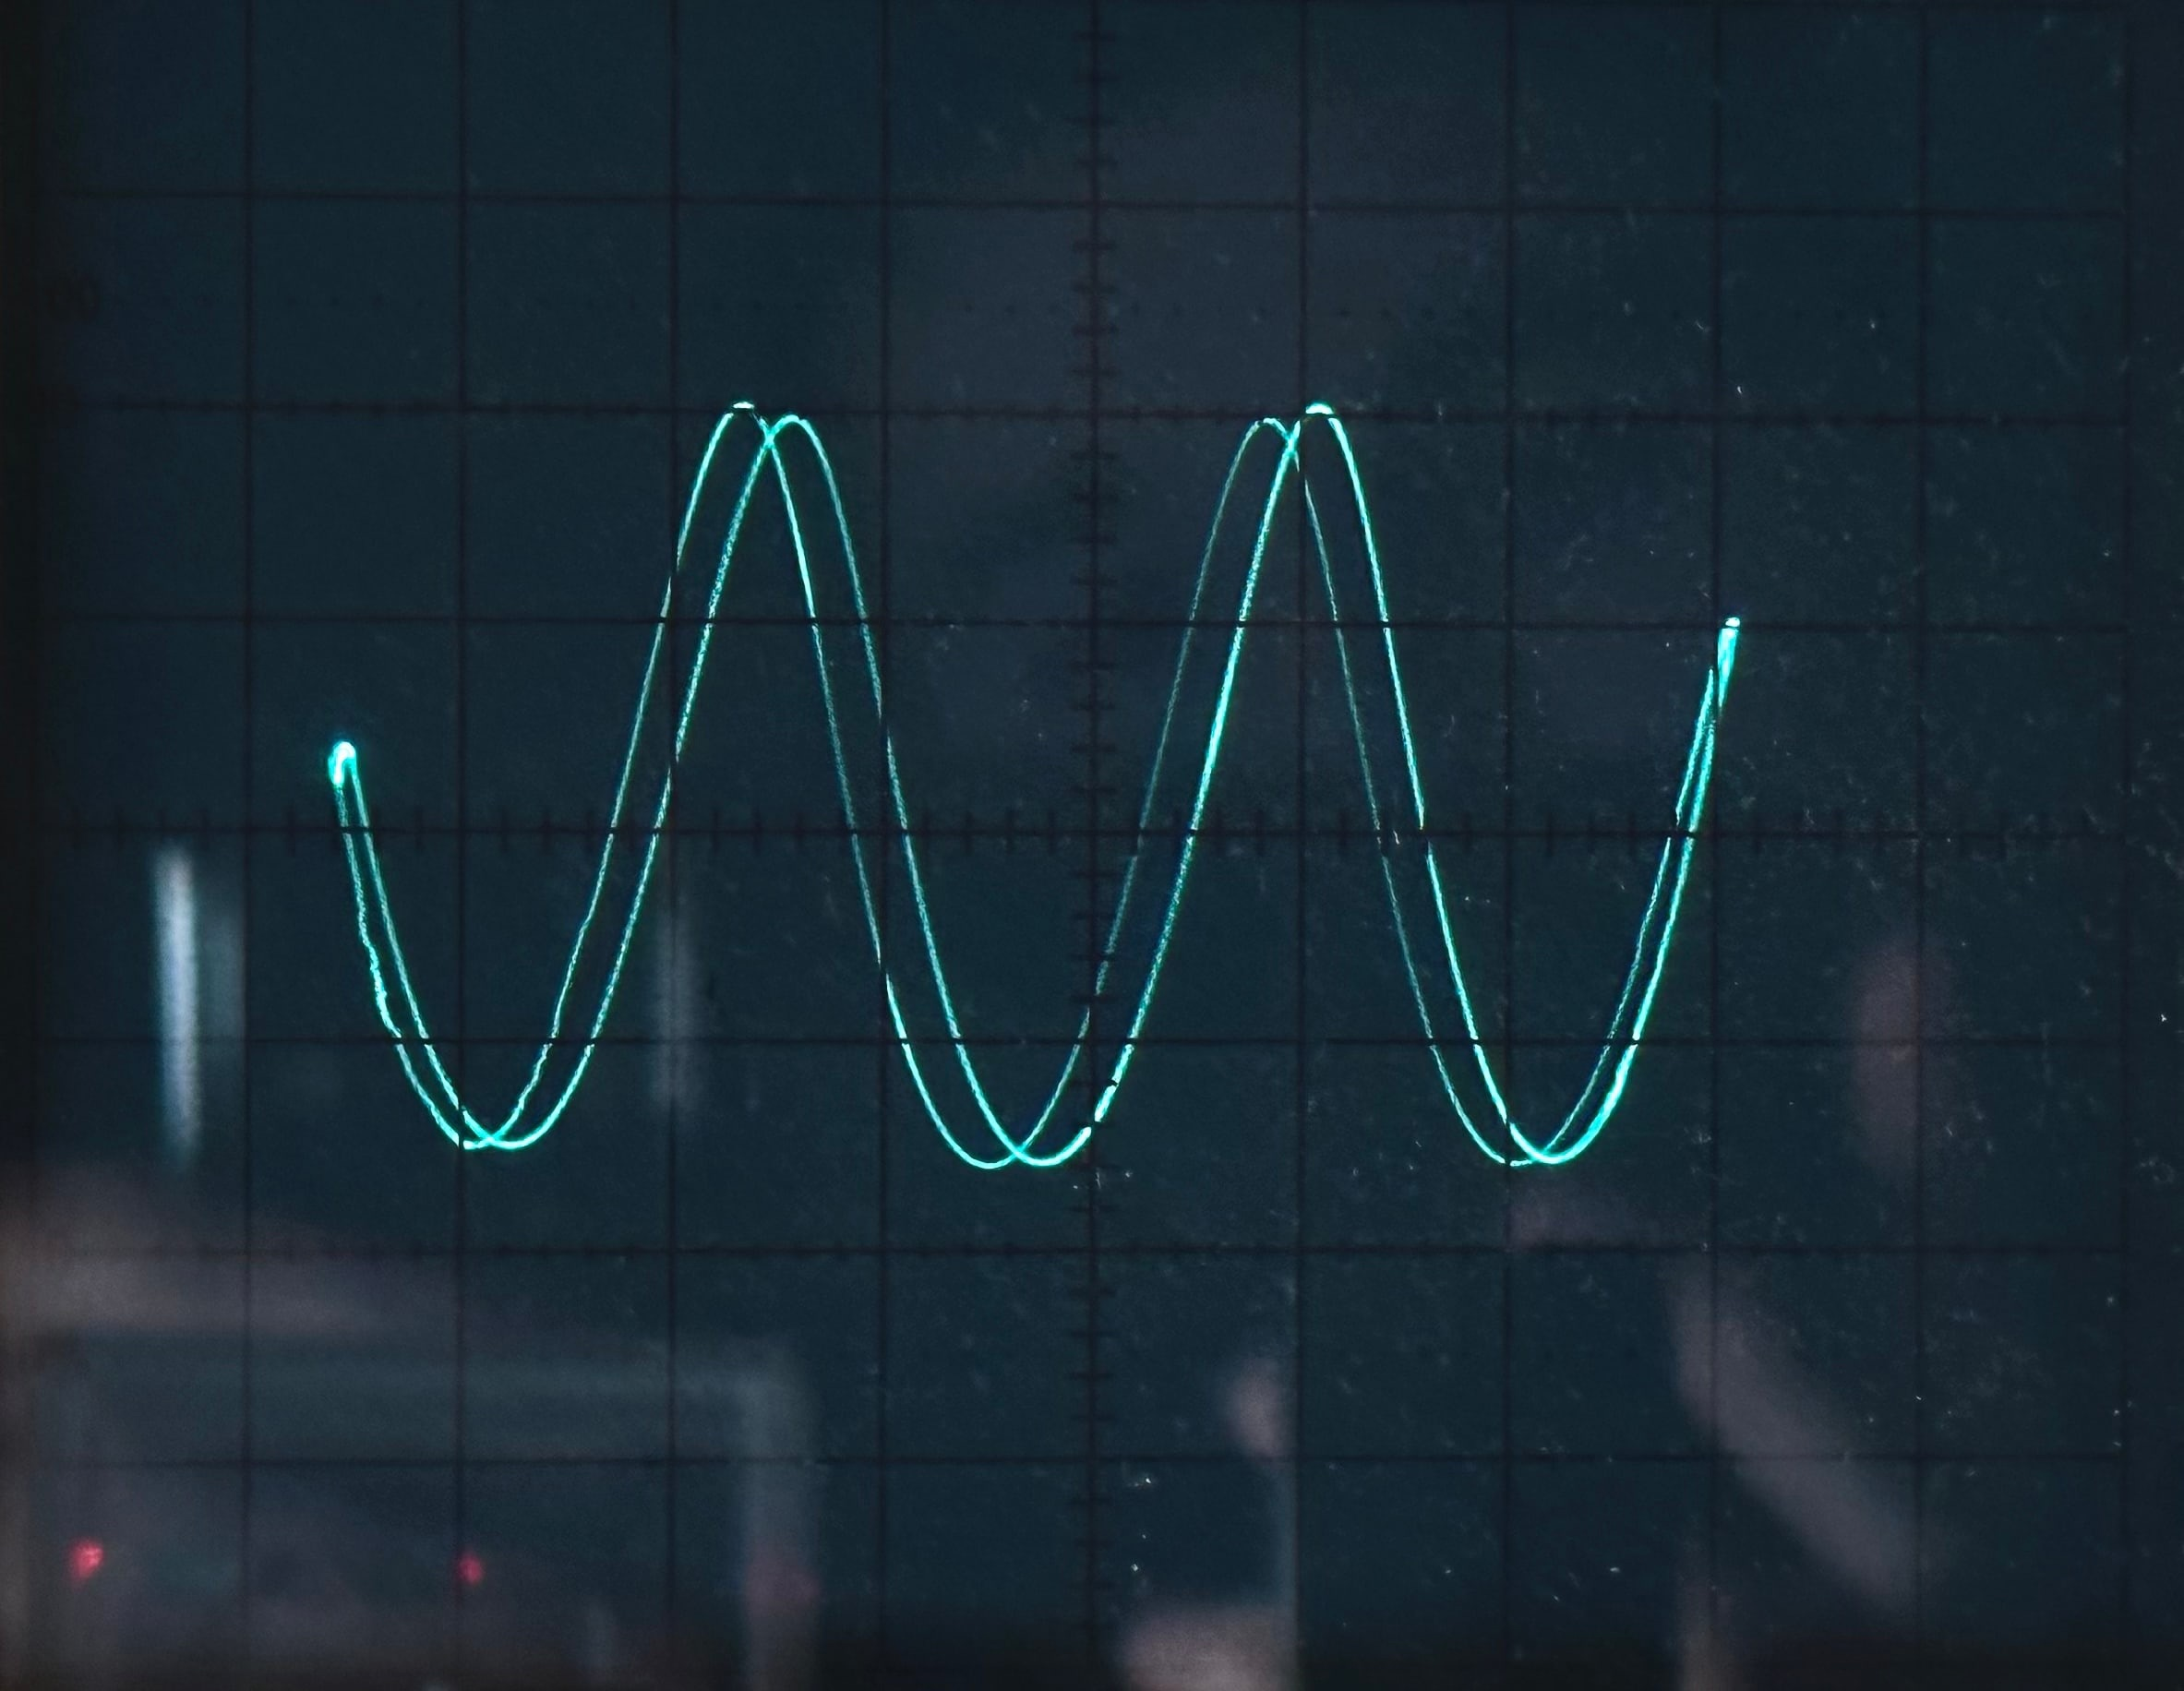
\includegraphics[width=0.9\linewidth]{cos3.jpg} \\ c)}
		\end{minipage}
		\caption{Фигуры Лиссажу для параллельных поляризаций при различных амплитудах напряжения $U$: (a) $U = U_{\lambda/2}$, (b) $U = U_{\lambda}$, (c) $U = U_{3\lambda/2}$ }
		\label{lis}
	\end{figure}
	
\newpage

\section{Обсуждение результатов и выводы}

В данной работе было определено двулучепреломление ниобата лития, полученное значение:
$$\boxed{n_o - n_e = (94,5\pm1,5) \cdot 10^{-3}}$$
Полученное значение согласуется с табличным ($n_o - n_e = 0,089$) в пределах $3\delta$. Основной вклад в погрешность вносит ошибка определения радиуса колец на экране.

%С помощью подачи на кристалл постоянного напряжения был получен свет, поляризованный по кругу. Это было определено при вращении анализатора, так как при этом яркость пятна на экране не изменялась.

Также двумя способами было определено полуволновое напряжение кристалла ниобата лития: по изменению яркости пятен на экране при вращении анализатора (при постоянном напряжении на кристалле) и по фигурам Лиссажу на экране осциллографа при переменном напряжении на кристалле. Полученное вторым способом значение:
$$\boxed{U_{\lambda/2} \approx 450~B}$$
согласуется со значениями, полученными первым способом.

\end{document}
